\documentclass[a4, 12pt]{article}
\usepackage{graphicx}
\usepackage{hyperref}
\usepackage{datatool}

\begin{document}
\section{Introduction}
%Need to finish introduction
Inferring glacier thickness has been a problem for a long time for glaciologists. This data is necessary for determining the total volume of ice for a given glacier outline, but also for modelling glacier flow.
Acquiring such data is hard and rather complicated given the wild nature of the fieldwork for glaciologists. Drilling a borehole trough a glacier is long and necessitate cumbersome machinery.\\

Hence the development of indirect methods such as geophysical and remote-sensing methods.

As part of an Undergraduate scolarship research award project, I will be helping two master's students, Tryggvi Unnsteinsson and Andrew Nolan, who are modelling ice flow of two glaciers in western Canada. The goal of this project is to review different ice thickness models and ultimately to infer bed topography for the two studied glaciers.

\section{The glaciers studied}
% Really unnamed or called little glacier? See: https://www.pc.gc.ca/en/pn-np/yt/kluane/nature/surge

% Are those section needed as they will be more extensively covered in the masters projects?
The glaciers under study are Job glacier, which is located on Mt. Meager in southwestern British Columbia  and an unnamed surging glacier part of the bigger Kluane glacier, in southern Yukon. Various data is available for each one. The next section will go over what is available for each glacier.\\

To note: further writing will be made here.

\subsection{Job glacier}
% Located on mt meager or mt job?
% Need to finish section
Job glacier is located upon Mt. Meager, a volcano in southwestern British Columbia. The hypsometric curve of Job glacier is shown at figure \ref{fig:job_hypso}.\\
The data available for Job glacier consists of a LIDAR survey from (?) and a glacier outline taken from Randolh Glacier Inventory. Also available is ice thickness data from a ground penetrating radar campaign held by Dr. G. Flowers and her team in September 2018. 



\subsection{Little Kluane}
% Need to finish section
The hypsometric curve of Little Kluane is shown at figure \ref{fig:lk_hypso}. The data available consists of a digital elevation model (?) and a glacier outline from Nolan(2020). 


\section{The Ice Thickness Models Intercomparison eXperiment, ITMIX}
The ever growing supply of different ice thickness models called for the need of a unified intercomparison experiment. The Ice Thickness Models Intercomparison eXperiment, ITMIX, is a project launched by the working group on glacier ice thickness estimation, part of the International Association of Cryospheric sciences.\\
The experiment consists of 17 different models tested over 21 cases, providing at least, depending on data availability:
\begin{itemize}
\item a glacier outline
\item a digital elevation model
\end{itemize}
And a combination of:
\begin{itemize}
\item the surface mass balance
\item the velocity field
\item the rate of ice thickness change
\end{itemize}
There were 4 main types of models trough this experiment:
\begin{itemize}
	\item Minimization approaches
		\begin{itemize}
			\item Those models defines ice thickness inversion as a minimization problem. They use a cost 					function consisting of minimizing the difference between observed and modelled data. 						The models presented in ITMIX all need the glacier outline, a digital elevation model 					and distributed surface mass balance.
		\end{itemize}
	\item Mass conserving approaches
		\begin{itemize}
			\item These methods are based on the principle of mass conservation (Farinotti, 2020). The 						ice flux divergence has to be compensated by the rate of ice thickness change and the 						climatic mass balance:
				\[\nabla \cdot q = \frac{\partial h}{\partial t} - \dot{b}\]
				To note is that most of the models in this category use the least amount data, only						needing the glacier outline and the digital elevation model.
		\end{itemize}
	\item Shear-stress based approaches
		\begin{itemize}
			\item Those approaches rely on some estimation of the basal shear stress $\tau$. They then 					solve for ice thickness using the shallow ice approximation (Fowler and Larson, 1978)
			\[h = \frac{\tau}{f\rho g \sin{\alpha}}\]
			An important thing to note is that those models don't take into account mass conservation. 					They then don't need much data to be able to produce a working model, only needing the 						glacier outline and a digital elevation model.
		\end{itemize}
	\item Velocity-based approaches
		\begin{itemize}
			\item The models described in this category are based on a form of Glen's flow law (Glen, 					1955) and an approximation of either the basal velocity $u_b$ or the depth-averaged profile 				velocity $\bar{u}$ from the surface velocity $u_s$. Those models all need the surface 						velocity field, the glacier outline a the digital elevation model.
		\end{itemize} 
	\item Other approaches
		\begin{itemize}
			\item GCneuralnet(Clarke et al., 2009) is a model based no artificial neural networks. It is based on the assumption that the bedrock topography resembles nearby unglaciarized valleys. This model only needs the glacier outline and the digital elevation model.
			\item Brinkerhoff (Brinkerhoff et al., 2016) is based on the Bayesian inference. The idea is that the bed elevation and the ice flux divergence can be described as Gaussian random fields with known covariance but unknown mean. This model can only work for the glaciers where all the data offered in ITMIX is available.
		\end{itemize}		
\end{itemize}
As there is little data available for the glaciers under study, Job and Little Kluane, it is important to choose a model corresponding to potentially accessible data. ITMIX concluded that the models using the most data weren't always the best representation of actual bedrock topography. This is probably caused by the high variation in the methodology used by various scientists to capture such data. Thus the lack of surface velocity field or rate of ice thickness change over time data isn't too dramatic.

ITMIX ranked the models from best to worst according to their performance over two rankings:
\begin{itemize}
	\item Their performance over the glaciers they tested.
	\item Their performance over all the glaciers, considering the amount of test-cases. 
\end{itemize}
It is however important to note the individual performance of the models when inferring ice thickness of similar glaciers to our study sites, considering location and topography, thereby the need of quantifying similarity in glacier geometry.

\section{Comparing glacier geometry}
% Need to go over the way hypsometry was computed
The hypsometric curve is defined by the elevation in relation to relative surface area from a defined location. In such, the hypsometric curve of a definer glacier outline relates the percentage of area over a given elevation. By using relative elevation over absolute elevation, we can quantify similarity between different hypsometric curves.
Those curves can be seen in figures \ref{fig:job_hypso} and \ref{fig:lk_hypso}.

\begin{figure}[h!]
	\centering
	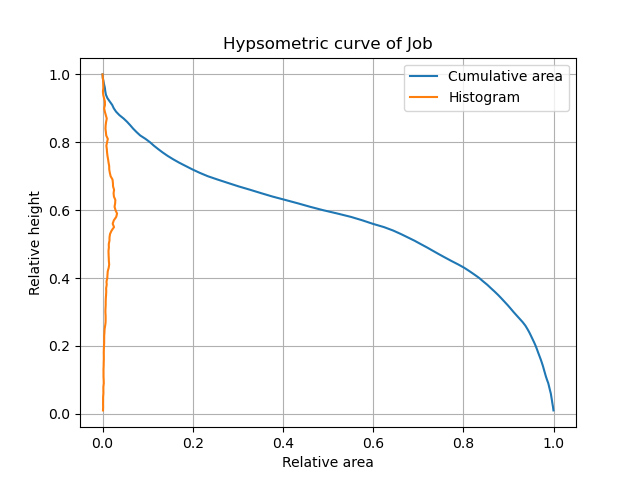
\includegraphics[scale=0.5]{../hypsometric_curves/Job_hypso.png}
	\caption{Job glacier's hypsometric curve}
	\label{fig:job_hypso}
\end{figure}

\begin{figure}[h!]
	\centering
	\includegraphics[scale=0.5]{../hypsometric_curves/Little kluane_hypso.png}
	\caption{Little Kluane's hypsometric curve}
	\label{fig:lk_hypso}
\end{figure}
% How to compare the shape and geometry? 
The topography of ITMIX's glaciers are compared to Job's and Little Kluane's by computing their hypsometric curve and using the values of percentile area corresponding to percentile elevation such that:
\begin{equation}
\%_{Area} = f(\%_{Elevation})
\end{equation}
If two glaciers were identical, plotting their $\%_{Area}$ in function of the other would give us points lying on the $x=y$ line. Thus, because the $\%_{Area}$ values are distributed equally on $\%_{Elevation} $ between $ [1,100]$, we can compare two glaciers by computing a statistical coefficient 
\begin{equation}
% Ok this really could be rewritten in a better way
R^2 = 1 - \frac{\sum(\%_{Area_x} - \%_{Area_y})^2}{\sum(\%_{Area_x} - \bar{\%_{Area_x}})^2}
\end{equation}

A higher value of $R^2$ would mean a higher resemblance between the overall topography of the glaciers.
The top correlations of each glaciers were compiled and ranked in Table \ref{tab:glacier_correl}\\
\DTLloaddb{rs}{../hypsometry_compared_r2_ez_view.csv}

Those glaciers are the better correlated to our study cases. Their hypsometric curves can be seen in the appendix. More data would be interesting to look at for better comparison:
\begin{itemize}
	\item The actual geometry of the glacier has been mostly ignored. It would be great to be able to quantify similarity in the shapes of the glacier.
	\item Other attributes such as the length, the slope or the equilibrium line altitude were ignored. 
	\item The histogram was computed. It seem to not work completely though, the histogram values are very small. It would be great to see if the similarity between the histograms and the hypsometric curve are the same.
\end{itemize}


\section{Comparing Itmix models}
In order to see what models fared better for those glaciers, the error of every model was computed. The error $\epsilon$ is computed like this:
\[\epsilon = h - h'\]
Since the $h$ data are points, the error is local and no heat maps were produced. No interpolation between the points for distributed ice thickness was made in order to obtain the "truest" error.
The relative error $\epsilon_\%$ was computed like this:\\
% This really doesn't look right
\[\epsilon_\% = 100\frac{\epsilon}{h}\]

The mean, the standard deviation, the minima, maxima and the absolute maxima of the error was computed and used as a metrics. Other metrics could and will be used for further investigation of the better models:
\begin{itemize}
\item Mean square error $MSE = \frac{1}{n}\sum{\epsilon^2}$
\item $R^2$ coefficient
\end{itemize}

The ice thickness of every computed model for each glacier was plotted along with its error. Such a figure is seen at figure \ref{fig:ng_error}.
\begin{figure}[h!]
	\centering
	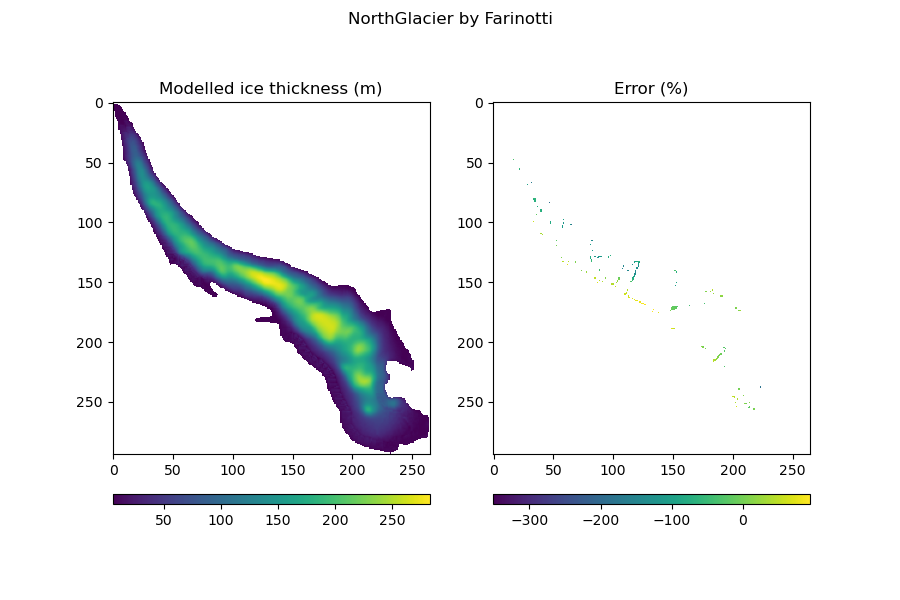
\includegraphics[scale=0.5]{../comparison_images/NorthGlacier_Farinotti_error.png}
	\caption{NorthGlacier's modelled ice thickness by Farinotti and its error}
	\label{fig:ng_error}
\end{figure}
A few problems remain with the picture:
\begin{itemize}
\item The shapefile hence the geometry of the glacier cannot be seen on the error map. This is a problem being investigated.
\item The error cannot be seen well on every map because of the nature of the data, which are points. This problem is also being looked at.
\item The $x$ and $y$ axis needs to be the coordinates of the glaciers.
\item The error computed seems quite big, verification of the computing needs to be made.
\end{itemize}
\section{What's next}
Further investigation will be made to quantify similarity in glacier geometry mainly with:\\
\begin{itemize}
	\item The shape of the glaciers. Some interesting ressources can be found here:
	\begin{itemize}
		\item \url{http://agri.ckcest.cn/ass/NK005-20160725003.pdf}
		\item \url{https://www.student.cs.uwaterloo.ca/~cs763/Projects/phil.pdf}
	\end{itemize}
	\item Their more basic geometry, such as length, width, mean slope and ELA
	\item Making sure the histogram computed is right and comparing their shape the same way it was made with the hypsometric curve
\end{itemize}
Verification of the error computed for every model and glacier will be made. The error maps will also be adjusted to add the contour of the glaciers and correctly see the error distribution.\\
\\
When the error is correctly computed and the similarity in glaciers will be better quantified, the best performing model from the chosen metric, either:
\begin{itemize}
\item $R^2$ coefficient
\item $MSE$
\item Mean error
\item and more!!
\end{itemize}
will be selected and the inferring work will finally begin...

\end{document}
